\chapter{System Design}


\section{Framework Of Medora}
\label{sec:Framework of Medora}
The framework of Medora involves three primary components: \textbf{Input}, \textbf{Process}, and \textbf{Output}. These components work together to ensure the seamless operation of the robot and its ability to provide personalized and adaptive care to elderly users.

\subsection*{Input}

\begin{itemize}
    \item \textbf{User Voice Commands and Facial Recognition Data:} The robot receives input from users through voice commands and facial recognition, enabling it to identify individuals and respond to their specific needs.
    
    \item \textbf{Environmental Sensor Data:} Equipped with sensors, the robot gathers environmental data such as room temperature, which supports real-time health monitoring.
    
    \item \textbf{Predefined Medication Reminders:} The system receives input in the form of scheduled medication plans, allowing the robot to provide timely and accurate notifications to users.
\end{itemize}

\subsection*{Process}

\begin{itemize}
    \item \textbf{AI-Powered Facial Recognition and Emotion Detection:} The robot employs deep learning models such as DeepFace and face cascade classifiers to perform accurate facial recognition and emotion detection. This allows it to tailor interactions based on user identity and emotional state.
    
    \item \textbf{Voice Recognition and Natural Language Understanding:} Natural Language Processing (NLP) enables the robot to interpret spoken commands and engage in meaningful, intuitive conversations with users.
    
    \item \textbf{Real-Time Health Data Monitoring:} IoT-based sensors integrated into the robot continuously monitor body temperature and provide real-time health updates to support elderly users' well-being.
\end{itemize}

\subsection*{Output}

\begin{itemize}
    \item \textbf{Visual and Audio Feedback:} The robot interacts with users through voice responses and screen-based visual cues, ensuring a user-friendly and accessible experience.
    
    \item \textbf{Medicine Reminders and Health Monitoring Updates:} The robot actively issues reminders for medication intake and shares real-time health updates, enabling better self-management of health conditions.
\end{itemize}
\begin{figure}[h]
    \centering
    % Replace the path and filename with your actual image
    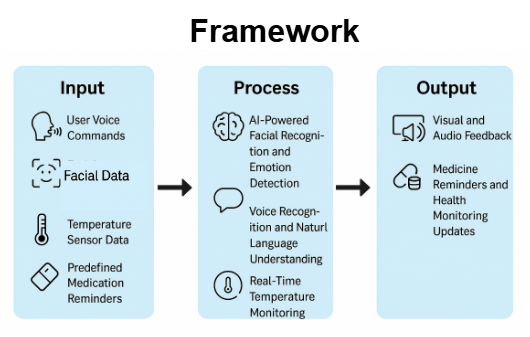
\includegraphics[width=0.8\textwidth]{Medora_thesis (1)/pics/thesis/abcde.png}
    \caption{ Framework of Medora}
    \label{fig:Framework Of Medora}
\end{figure}

\section{Overview of Medora System Design}

The Smart Medora is engineered to deliver integrated healthcare support and intelligent interaction, particularly tailored for elderly individuals in home or assisted living environments. The system design centers around a compact and efficient framework built on the \textbf{Raspberry Pi 4B}, combining facial recognition, emotion detection, voice-based communication, temperature monitoring, and emergency response. It integrates multiple hardware and software components to provide real-time care, emotional support, and personalized interaction, all within a modular and cost-effective setup.


The\textbf{Block Diagram} of Medora  :
\begin{figure}[h]
    \centering
    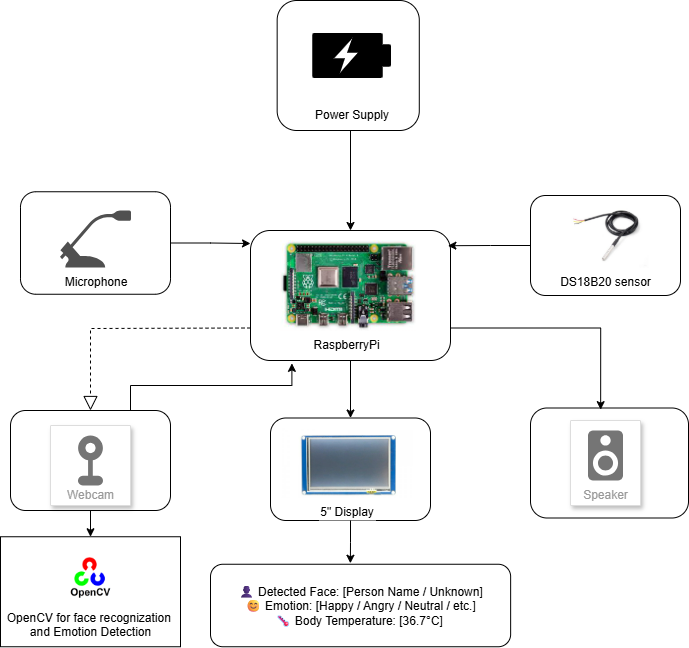
\includegraphics[width=0.5\textwidth]{Medora_thesis (1)/pics/thesis/bdm2.png} % Replace with your actual image filename
    \caption{Block Diagram of Medora}
    \label{fig:Block Diagram of Medora}
\end{figure}

\subsection{General Overview of Medora}

Smart Medora employs a multi-layered approach to user interaction by combining facial recognition, emotion analysis, and real-time voice communication. Utilizing a USB webcam and the \texttt{face\_recognition} library, Medora accurately identifies users from a stored facial database, ensuring that only authorized individuals can access sensitive health-related features like temperature monitoring or medication schedules.

Once a user is authenticated, Medora conducts emotional analysis using the DeepFace library. This feature enables it to interpret basic affective states such as happiness, sadness, anger, or neutrality. Based on these emotional cues, Medora dynamically tailors its verbal responses, allowing for more empathetic and context-aware conversations.

Medora also integrates physical health monitoring via the \texttt{DS18B20} digital temperature sensor connected to GPIO4. It periodically logs temperature readings, identifies anomalies, and issues alerts when predefined thresholds are exceeded. Voice interactions are enabled through a microphone and powered by Google's Speech-to-Text API. Intelligent, human-like responses are generated using OpenAI’s GPT API and vocalized using the \texttt{gTTS} engine through a connected speaker, creating a seamless conversational loop for delivering reminders, health advice, and emotional support.emotional support.

\subsection{Structural Characteristics of Medora}


Medora stands out as a lightweight, modular, and cost-effective assistive robot tailored for elderly care, with a strong emphasis on accessibility and emotional responsiveness. The system is powered by a Raspberry Pi 4B and integrates essential hardware modules such as a webcam, temperature sensor, microphone, speaker, and an optional 5” HDMI display.

Its local processing capabilities allow for face detection and recognition, even without continuous internet access, ensuring reliable identity-based personalization. In addition, Medora uses lightweight AI models for emotion detection, enabling it to respond with empathy—offering comforting words or proactive support based on the user's visible emotional state.

Unlike traditional medication dispensers or monitoring devices, Medora delivers a holistic care experience. It combines regular temperature tracking with intelligent reminders for medicine intake, hydration, or medical checkups. These reminders can be both scheduled and voice-activated, creating an intuitive and user-friendly interface.

The architecture supports a hybrid operational model where local processing ensures core functionalities (face recognition, temperature sensing) remain available during connectivity issues, while cloud services handle advanced conversation and language tasks. This thoughtful integration of hardware and AI enables Medora to operate as a dependable, emotionally aware companion for older adults in both home and institutional settings.

\subsection{Interactive Features and Interface Design}


The interactive design of the Smart Medora follows user-centric principles focused on elderly accessibility. It features a simplified voice-first interface that eliminates the need for manual interaction. Users can speak naturally to the system, and the Medora responds in a human-like voice, offering medication reminders, motivational prompts, or conversational responses depending on the context and emotional state.

The optional 5” display can visually present the UI, such as video feeds, health status, or alerts, and can be particularly helpful during setup or for caregivers. The system supports multilingual voice synthesis, adaptive volume control based on ambient conditions, and is capable of initiating interactions without user input—creating a proactive care experience. Over time, the AI tailors its interactions to individual users, adapting its tone and content to provide familiarity, emotional comfort, and companionship.


A logical Architectural Diagram of Medora is given Below :
\begin{figure}[h]
    \centering
    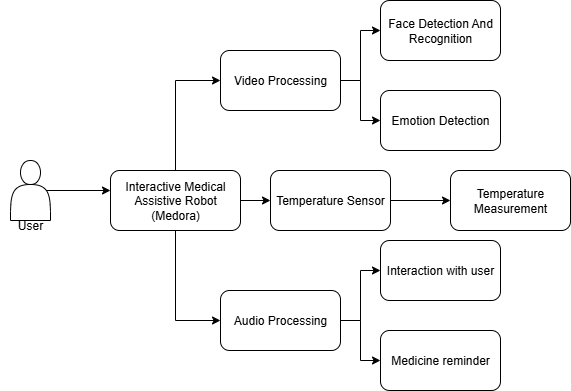
\includegraphics[width=0.8\textwidth]{Medora_thesis (1)/pics/thesis/lad.png} % Replace with your actual image filename
    \caption{Logical Architecture Diagram}
    \label{fig:Logical Architecture Diagram}
\end{figure}





\section{Hardware Components}

The \textbf{Smart Medora } incorporates a well-selected collection of hardware components that focus on delivering effective functionality, reliability, and affordability. The system consists of computational, sensing, communication, and user interface components to support its aim of elderly care, monitoring, and interaction. Provided below is the detailed decomposition of the key hardware utilized in developing the Medora :

\subsection*{Microcontroller}

\textbf{Raspberry Pi 4B} \\
A versatile, low-cost single-board computer capable of supporting complex tasks such as data processing, sensor integration, and multimedia communication. With its quad-core processor, GPIO pins, and wireless connectivity, the Raspberry Pi 4B is ideal for managing real-time operations, AI algorithms, and user interaction in robotics and automation systems.

\begin{figure}[H]
    \centering
    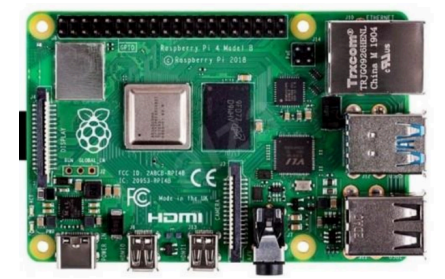
\includegraphics[width=0.8\textwidth]{pics/thesis/raspberry.png}
    \caption{Raspberry Pi 4B (Microcontroller)}
    \label{fig:raspberry_pi}
\end{figure}


\subsection*{Webcam}

\textbf{Webcam (USB)} \\

The system includes a USB webcam that connects via a standard USB interface, providing visual input for various applications such as video monitoring, image processing, computer vision, or user interaction. The webcam captures live video or still images and transmits them to the processing unit in real time, enabling functionalities like facial recognition, object detection, or remote observation. Depending on the model, the webcam may offer features such as HD or Full HD resolution, autofocus, low-light enhancement, and built-in microphones. Its plug-and-play USB connectivity ensures broad compatibility with most operating systems and embedded platforms, making it a flexible and essential component for systems that require visual data capture.

\begin{figure}[H]
    \centering
    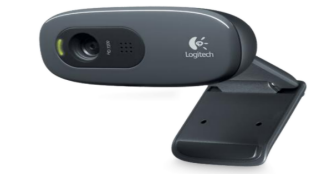
\includegraphics[width=0.5\textwidth]{pics/thesis/webcam.png}
    \caption{Webcam}
    \label{fig:Webcam}
\end{figure}

\subsection*{Microphone}

\textbf{Wired Microphone} \\

The system includes a wired microphone that serves as an audio input device for capturing sound, voice commands, or ambient audio signals. Typically connected via a 3.5mm audio jack or USB interface, the microphone enables functionalities such as voice control, audio recording, speech recognition, or real-time communication. It is particularly useful in applications involving user interaction, sound-based monitoring, or integration with AI voice assistants. The wired connection ensures a stable and low-latency audio signal, making it suitable for embedded systems, IoT devices, or robotics platforms that require consistent and accurate audio input. Depending on the design, the microphone may be omnidirectional or unidirectional, and often includes basic noise reduction features to enhance clarity in various environments.

\begin{figure}[H]
    \centering
    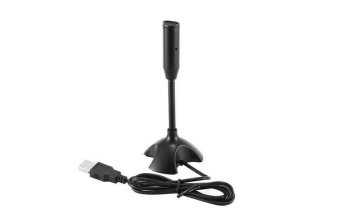
\includegraphics[width=0.4\textwidth]{pics/thesis/microphn.png
}
    \caption{Microphone}
    \label{fig:Microphone}
\end{figure}

\subsection*{Speaker}

\textbf{Speaker (AUX Port)} \\

The system includes an external speaker connected via a standard 3.5mm AUX port, providing audio output for applications that require sound feedback, alerts, or spoken instructions. This setup enables the device to play system notifications, voice prompts, or multimedia content, depending on the software configuration. The AUX port ensures compatibility with a wide range of passive and powered speakers or headphones, offering flexibility in audio output options. Whether used for basic alert tones or more advanced voice interaction, the speaker enhances user experience by adding an auditory layer to the system’s interface.

\begin{figure}[H]
    \centering
    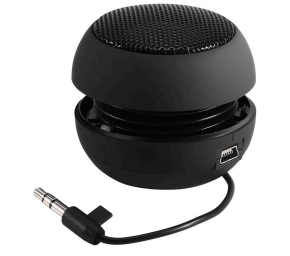
\includegraphics[width=0.4\textwidth]{pics/thesis/speaker.png
}
    \caption{Speaker}
    \label{fig:Speaker}
\end{figure}

\subsection*{Display}

\textbf{5” Display (Micro HDMI)} \\

The 5” display connected via a Micro HDMI port serves as an optional visual interface for the system, providing real-time output of video feeds or user interfaces depending on the application. This compact screen is especially useful in scenarios where monitoring, configuration, or user interaction is required directly on the device. It is commonly used in embedded systems, robotics platforms, and IoT solutions to display live camera feeds, system diagnostics, graphical menus, or operational data. In some configurations, it also supports touchscreen input, allowing for interactive control without the need for external peripherals. The Micro HDMI interface ensures high-quality digital video transmission from the main processing unit, such as a Raspberry Pi, Jetson Nano, or similar board, while power is generally supplied through a separate USB connection. Although it enhances usability, the display is optional and the system can operate in a headless mode or be accessed remotely, making it a flexible component suited for both development and deployment environments.



\begin{figure}[H]
    \centering
    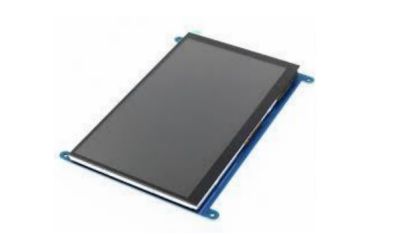
\includegraphics[width=0.7\textwidth]{pics/thesis/display.png
}

    \caption{5-Inch Raspberry Pi Touchscreen Display
}
    \label{fig:5-Inch Raspberry Pi Touchscreen Display
}
\end{figure}


\subsection*{Power}

\textbf{Power (5V USB-C Adapter)} \\

The system is powered using a 5V USB-C adapter, which serves as the primary power source for all components. This power input ensures a stable and efficient energy supply, capable of supporting both the core processing unit and any connected peripherals, such as displays, sensors, and communication modules. The use of a USB-C connector offers modern compatibility, improved current handling, and ease of connection compared to older power standards. Delivering 5 volts, the adapter is typically rated to supply sufficient current—often 2.5A to 3A or higher—depending on the system’s total power consumption. This setup allows for consistent performance and reliable operation across various applications, including embedded, robotics, and IoT environments.


\begin{figure}[H]
    \centering
    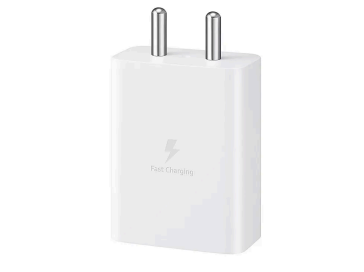
\includegraphics[width=0.5\textwidth]{pics/thesis/adapter.png}
    \caption{Adapter}
    \label{fig:Adapter}
\end{figure}


\subsection*{Filament (Body Construction)}

\textbf{PET-G Filament} \\

 Used in the 3D-printed structure of the robot, PET-G filament offers durability, excellent layer adhesion, and resistance to impact and moisture. It is especially well-suited for environments where robustness and aesthetics are both important.

 
\begin{figure}[H]
    \centering
    
\includegraphics[width=0.5\textwidth]{pics/thesis/filament.png}
    \caption{Filament}
    \label{fig:Filament}
\end{figure}


\subsection*{Temperature Sensor}

\textbf{DS18B20 Sensor} \\

The DS18B20 is a digital temperature sensor that provides accurate readings (±0.5°C) from -10°C to +85°C, and up to -55°C to +125°C. It uses the 1-Wire protocol, allowing multiple sensors on a single data line, and each sensor has a unique 64-bit ID for identification. It supports parasite or external power (3–5.5V) and outputs digital data directly, making it ideal for microcontroller-based systems. Common applications include weather stations, environmental monitoring, HVAC, and industrial control.

\begin{figure}[H]
    \centering
    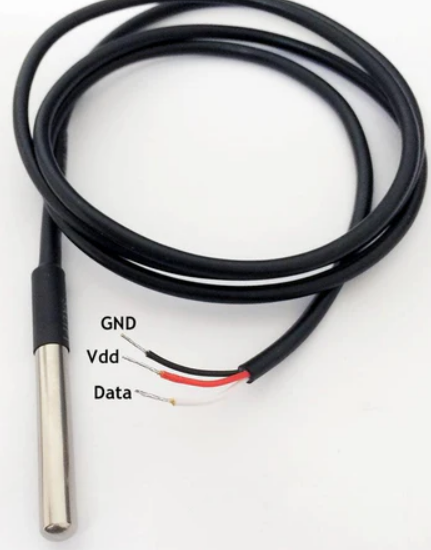
\includegraphics[width=0.4\textwidth]{pics/thesis/Screenshot 2025-06-03 124407.png}
    \caption{Digital Temperature Sensor}
    \label{fig: Digital Temperature Sensor}
\end{figure}


\subsection*{Voltage Regulator}

 \textbf{Power Voltage Regulator} \\

Ensure consistent and safe voltage levels to protect microcontrollers, sensors, and other sensitive electronic components. This regulator stabilizes power delivery, preventing system errors or hardware damage due to fluctuations.

\begin{table}[H]
\centering
\caption{Components List with Specifications and Cost}
\begin{tabular}{|l|p{7cm}|r|}
\hline
\textbf{Components} & \textbf{Specification} & \textbf{Price List (BDT)} \\
\hline
Raspberry Pi 4B & Quad-core processor, GPIO pins, Wi-Fi connectivity & 14,994 \\
\hline
Webcam (USB) & HD resolution, USB 3.0 interface for real-time video capture & 2,500 \\
\hline
Microphone & USB/3.5 mm audio jack or USB interface for voice input & 500 \\
\hline
Speaker (AUX Port) & 3.5mm AUX connection for audio output & 800 \\
\hline
5" Display (Micro HDMI) & Touchscreen, 800x480 resolution, optional for UI feedback & 3,000 \\
\hline
Power (5V USB-C Adapter) & 5V, 3A power supply for stable operation & 600 \\
\hline
PET-G Filament & Durable material for 3D-printed body enclosure & 2,200 \\
\hline
DS18B20 Sensor & Digital temperature sensor with ±0.5°C accuracy, 1-Wire protocol & 300 \\
\hline
Power Voltage Regulator & Stabilizes voltage to protect sensitive components & 400 \\
\hline
\end{tabular}
\label{tab:components_cost}
\end{table}

\section{Software Design }

\subsection{Facial Recognition Module}
The system uses the \texttt{face\_recognition} library (built on dlib) to detect and identify known individuals from video frames. Prior to execution, images of known individuals are stored in labeled folders. These are loaded, encoded into 128-dimensional facial vectors, and compared in real time against faces detected from video input using Euclidean distance. A match is declared if the distance falls below a threshold (0.45).

\subsection{Emotion Detection System}
To maintain real-time performance, the system employs the DeepFace library, which utilizes deep convolutional neural networks (CNNs) to analyze facial expressions and classify them into basic emotions such as happy, sad, or angry. For each detected face, a cropped image of the face region is processed by DeepFace, and the dominant emotion is determined based on the highest confidence score.

\subsection{AI Chatbot Integration}
The emotional state and name of each recognized individual are embedded into a natural language prompt. This prompt is sent to a GPT-based chatbot model via the OpenRouter API. The model (e.g., gpt-3.5-turbo) generates a short, personalized response based on the input. This approach eliminates the need for manual scripting by allowing dynamic sentence generation tailored to each person’s identity and emotion.

\subsection{Voice Interaction and Feedback}
The generated text is converted into speech using the \texttt{pyttsx3} offline TTS engine. To avoid robotic-like delays (often caused during speech generation), a multithreaded approach is used, ensuring that video capture and emotion processing continue while speaking.

\subsection{ Reminder System}
The reminder system enables the robot to provide timely notifications, such as medication or task reminders. Users can set reminders through natural voice commands, which are interpreted by the chatbot and converted into a structured schedule. Each reminder is stored with its message and target time. A dedicated background thread continuously monitors the schedule and triggers notifications using the text-to-speech engine when the scheduled time is reached. This multithreaded design ensures that reminders are delivered without interrupting ongoing face recognition, emotion detection, or voice interaction, providing seamless and reliable assistance to the user.
\subsection{ Temperature Measurement}
The system uses a DS18B20 temperature sensor connected via the 1-Wire protocol to monitor the user’s body or ambient temperature. The sensor readings are obtained in degrees Celsius and can be accessed in real time by the software modules. Temperature data is incorporated into the chatbot prompts and responses, allowing the assistant to provide context-aware guidance or alerts (e.g., notifying the user if the measured temperature is unusually high). This integration enhances Medora's ability to offer personalized health monitoring alongside emotional and conversational support.


\subsection{Overall System Flow and Logic}
The system operates in a sequential pipeline structure to ensure real-time performance, modularity, and contextual intelligence. The following steps detail the operational flow of the AI-driven facial and emotional recognition system.
\begin{enumerate}
    \item \textbf{Initialization}
    \begin{itemize}
        \item Predefined images of known individuals are loaded and encoded using the \texttt{face\_recognition} library.
        \item The emotion classifier (DeepFace)and text-to-speech engine (\texttt{pyttsx3}) are initialized.
        \item The OpenRouter GPT API key is set for chatbot integration.
    \end{itemize}

    \item \textbf{Video Input Handling}
    \begin{itemize}
        \item The system iterates through each video file located in the designated directory.
        \item Each video is read frame by frame using OpenCV. For performance, every second frame is selected for processing.
    \end{itemize}

    \item \textbf{Face Detection and Recognition}
    \begin{itemize}
        \item Each selected frame is resized to 25\% of its original dimensions to reduce computational load.
        \item Faces are detected, and facial encodings are extracted using the \texttt{face\_recognition} library.
        \item These encodings are compared with the known face dataset to identify the individual.
    \end{itemize}

    \item \textbf{Emotion Detection}
    \begin{itemize}
      
    \item For each detected face, the system crops the corresponding face region from the video frame.
    \item The cropped image is processed by the DeepFace library, which analyzes facial features to estimate emotion probabilities.
    \item The emotion with the highest confidence score is selected as the dominant emotional state.
\end{itemize}


    \item \textbf{Chatbot Prompt Construction and Querying}
    \begin{itemize}
        \item Once a person is recognized (and has not already been greeted in the current session), their name and emotion are embedded into a prompt.
        \item This prompt is sent to the OpenRouter GPT-based model (\texttt{gpt-3.5-turbo}) via HTTP POST request.
        \item The chatbot generates a brief, context-aware message addressing the individual and reflecting their emotional state.
    \end{itemize}


    \item \textbf{Response Vocalization}
    \begin{itemize}
        \item The chatbot response is converted to speech using \texttt{pyttsx3}.
        \item To prevent blocking the video stream during speech, the TTS process is run in a separate thread.
\end{itemize}
\end{enumerate}

\begin{figure}[H]
    \centering
    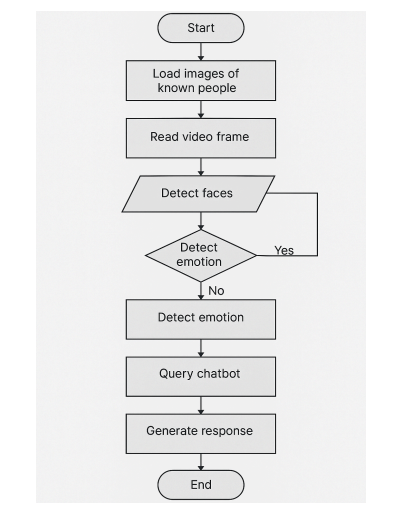
\includegraphics[width=0.5\textwidth]{pics/thesis/flowchart.png}
    \caption{Flowchart of Medora}
    \label{fig: Flowchart of Medora}
\end{figure}



\section{Methodology: Building Medora for Elderly Assistance}

The methodology of development for Medora, an inexpensive assistive robot that uses face recognition, emotion detection, voice interactions, and basic health monitoring to offer assistance to older populations, is presented in this section. Medora increases user engagement, encourages adherence to prescribed or suggested health routines, and helps establish a natural and accessible daily interaction—especially for older adults experiencing cognitive decline, loneliness, or lacking consistent caregiving. The methodology incorporates a user-informed design process, a modular hardware-software approach, and staged testing in environments that reflect real-world characteristics.

\subsection{Design and Physical Integration}

The development of Medora followed a human-centered design approach, prioritizing usability, accessibility, and non-intrusive support for elderly users in home and care environments. Initial surveys and user feedback helped identify critical needs, including personalized interaction, simple verbal communication, emotion recognition, and integrated temperature monitoring.  

Insights from these studies guided the design towards a friendly, passive presence rather than a humanoid form. The system emphasizes a compact, desk-sized, and modular structure that blends seamlessly into the user’s daily environment while providing contextual awareness through voice interaction and sensory feedback.

Physical integration focused on aligning hardware placement with user experience. Sensors, camera, microphone, and optional display were positioned to ensure accurate detection and comfortable interaction without obstructing the user. The casing was designed to be durable and resistant to environmental factors, while the overall assembly remains modular for easy maintenance and upgrades.  

This design approach ensures that Medora not only meets technical requirements but also aligns with the practical, emotional, and ergonomic needs of elderly users, forming a foundation for reliable and supportive interaction in daily life.


\subsection{Real-Time Interaction System: Software and Processing Pipeline}

Medora’s software system integrates multiple open-source libraries using Python to manage real-time face detection, emotion classification, chatbot interaction, and text-to-speech synthesis through a multi-threaded pipeline.

Major components include:

\begin{itemize}
    \item \textbf{Facial Recognition}: Utilizes \texttt{face\_recognition} (based on Dlib) for encoding and matching faces via Euclidean distance.
    \item \textbf{Emotion Detection}: Utilizes the DeepFace library, which leverages deep convolutional neural networks (CNNs) to analyze facial expressions and determine the dominant emotion, such as happy, sad, or neutral.
    \item \textbf{Conversational Response}: Sends dynamic prompts to a GPT-based chatbot (via OpenRouter API) incorporating user name and emotion.
    \item \textbf{Speech Output}: Uses \texttt{pyttsx3} for offline TTS; executed in a separate thread to avoid lag.
\end{itemize}

\textbf{Operational Flow:}
\begin{enumerate}
    \item Video frames are scanned for faces.
    \item Detected faces are compared to stored encodings.
    \item Emotion is inferred from the detected face.
    \item A context-aware text reply is generated and spoken.
\end{enumerate}

This structure ensures near real-time response, enabling fluid and natural interaction.

\subsection{Experimental Testing and Functional Validation}

To validate Medora’s practical performance, two stages of testing were performed:

\subsubsection*{Phase 1: Simulated Testing}
\begin{itemize}
    \item Evaluated facial recognition under different lighting and angles
    \item Tested emotion detection using datasets and real-time input
    \item Assessed voice interaction latency and chatbot relevance
\end{itemize}

\subsubsection*{Phase 2: Home-Style Deployment}
\begin{itemize}
    \item Medora was tested in a simulated home setting with elderly participants
    \item Evaluated interaction timing, recognition accuracy, and user response
    \item Iteratively improved misrecognition handling, emotional tone, and responsiveness
\end{itemize}

\textbf{Key Results:}
\begin{itemize}
    \item Facial recognition accuracy exceeded 90\% for known users
    \item Emotion detection succeeded for common emotional categories
    \item GPT-based replies rated as contextually appropriate and supportive
    \item Low error rate in TTS and temperature readings
\end{itemize}

\subsection{Spatial Deployment and Environmental Integration}

Medora is designed for fixed, spatially anchored deployment in locations frequented by older adults—such as desks, tables, or kitchen counters. This ensures reliable performance while maintaining a seamless fit in home environments.

Environmental design considerations include:

\begin{itemize}
    \item Optimized camera angles for seated users
    \item Effective voice pickup within a 2-meter radius
    \item PET-G casing with ventilation to support thermal and humidity variation
    \item No mobility included to avoid disrupting room layouts
\end{itemize}

Future versions may incorporate mobility or remote caregiver features (e.g., SMS alerts or health data syncing), based on feedback and further prototyping.

